\documentclass[11pt,a4paper,twoside,bibliography=totoc,listof=totoc,titlepage=true,chapterprefix=true]{scrreprt}

%% ---------------------------------------------------------------------------
%% Packages
%% ---------------------------------------------------------------------------

\usepackage[english]{babel} %Option: german für deutsche Variante
\usepackage[T1]{fontenc}   
\usepackage[utf8]{inputenc} 
\usepackage{lmodern}
%\usepackage{bibgerm}
\KOMAoptions{parskip=half, numbers=noenddot} 

\usepackage{amsmath}
\usepackage{amssymb}
\usepackage{graphicx}
\usepackage{subfig} % uses for subfloat: two pictues side by side
\usepackage{amsthm} % needed for proofs
\usepackage{multirow} % multirows for tables
\usepackage{placeins} % for floatbarrier
\usepackage{booktabs} % Für schönere wissenschaftliche Tabellen
\usepackage{tikz}
\usepackage[backend=biber, style=alphabetic]{biblatex} 
\usepackage[pdfpagelabels,hidelinks]{hyperref}
\usepackage{csquotes} % Wenn babel mit biblatex, dann wird csqoutes empfohlen, damit zitierter Text richtiges Typenset hat
\usepackage[numbered]{bookmark} % Für nummerierte PDF-Lesezeichen entsprechend der Chapter/Section-Nummer

\usepackage{geometry} % Einstellungen der Ränder 
\geometry{paperwidth=210mm, paperheight=297mm, height=247mm,width=167mm,top=21.5mm,right=15mm}%,headsep=7mm,headheight=10mm,footskip=11mm}
%\geometry{includehead,includefoot,inner=3cm,outer=2cm,top=2cm,bottom=2.5cm}

\usepackage{supertabular}
\usepackage{color} % Für farbige Boxen --> Gut für Notizen

\usepackage{xifthen}							% provides \isempty test

\usepackage[acronym,nonumberlist,section]{glossaries} % test this package

%\usepackage[ruled, vlined, linesnumbered,german]{algorithm2e}
\usepackage[ruled, vlined, linesnumbered]{algorithm2e}
\usepackage{listings}
\usepackage[headsepline, plainfootsepline]{scrlayer-scrpage}

%% ---------------------------------------------------------------------------
%% Definitions
%% ---------------------------------------------------------------------------

\newtheorem{theorem}{Theorem}[chapter]
\newtheorem{assumption}{Assumption}[chapter]

%% Heading styles
\RedeclareSectionCommand[%
		tocentryformat={\rmfamily\bfseries},%
		tocpagenumberformat=\rmfamily
	]{chapter}

\addtokomafont{part}{\rmfamily}
\addtokomafont{chapterprefix}{\huge\rmfamily}
\addtokomafont{chapter}{\Huge\rmfamily}
\addtokomafont{section}{\rmfamily}
\addtokomafont{section}{\rmfamily}
\addtokomafont{subsection}{\rmfamily}
\addtokomafont{subsubsection}{\rmfamily}
\addtokomafont{paragraph}{\rmfamily}
\addtokomafont{subparagraph}{\rmfamily}

%% Bibliography Styles
%\renewcommand{\mkbibnamefirst}[1]{\textsc{#1}}
%\renewcommand{\mkbibnamelast}[1]{\textsc{#1}}
%\renewcommand{\mkbibnameprefix}[1]{\textsc{#1}}
%\renewcommand{\mkbibnameaffix}[1]{\textsc{#1}}

%% Style for Algorithms
\newcommand{\listofalgorithmes}{\tocfile{\listalgorithmcfname}{loa}}
\SetKwRepeat{Do}{do}{while}%
\SetAlFnt{\small} %\SetAlFnt{\footnotesize }
\SetKwComment{Comment}{$\triangleright$\ }{}
\SetVlineSkip{2pt} 
\DontPrintSemicolon
\SetNlSty{}{}{:} % No Bold Line Numbers
\SetAlgoNlRelativeSize{-1} % relative Size of Line Number
\SetCommentSty{} % Sonst wäre Kommentar Fett    

%colorbox with line break
%background: colorbox adds some space before and after the text inside it, this space is \fboxsep
\newcommand{\hly}[1]{\colorbox{yellow}{\parbox{\dimexpr\textwidth-2\fboxsep\relax}{#1}}} 
\newcommand{\hlg}[1]{\colorbox{green}{\parbox{\dimexpr\textwidth-2\fboxsep\relax}{#1}}}
\newcommand{\hlr}[1]{\colorbox{red}{\parbox{\dimexpr\textwidth-2\fboxsep\relax}{#1}}}

%$ Listing Style
%% Listing Style for Matlab
\definecolor{mygreen}{rgb}{0,0.6,0}
\definecolor{mygray}{rgb}{0.5,0.5,0.5}
\definecolor{mymauve}{rgb}{0.58,0,0.82}
\lstset{numbers=left, numberstyle=\tiny, numbersep=5pt} \lstset{language=Matlab}
\lstset{basicstyle=\ttfamily}
\lstset{literate=%
	{Ö}{{\"O}}1
	{Ä}{{\"A}}1
	{Ü}{{\"U}}1
	{ß}{{\ss}}2
	{ü}{{\"u}}1
	{ä}{{\"a}}1
	{ö}{{\"o}}1
} 
\lstset{ %
	backgroundcolor=\color{white},   		% choose the background color; you must add \usepackage{color} or \usepackage{xcolor}
	basicstyle=\footnotesize,        					% the size of the fonts that are used for the code
	breakatwhitespace=false,         			% sets if automatic breaks should only happen at whitespace
	breaklines=true,                 								% sets automatic line breaking
	captionpos=b,                    								% sets the caption-position to bottom
	commentstyle=\color{mygreen},    	% comment style
	deletekeywords={...},            						% if you want to delete keywords from the given language
	escapeinside={\%*}{*)},          					% if you want to add LaTeX within your code
	extendedchars=true,              						% lets you use non-ASCII characters; for 8-bits encodings only, does not work with UTF-8
	frame=single,                    								% adds a frame around the code
	keepspaces=true,                 						% keeps spaces in text, useful for keeping indentation of code (possibly needs columns=flexible)
	keywordstyle=\color{blue},       				% keyword style
	language=Octave,                 						% the language of the code
	morekeywords={*,...},            						% if you want to add more keywords to the set
	numbers=left,                    									% where to put the line-numbers; possible values are (none, left, right)
	numbersep=5pt,                   						% how far the line-numbers are from the code
	numberstyle=\tiny\color{mygray}, 		% the style that is used for the line-numbers
	rulecolor=\color{black},         						% if not set, the frame-color may be changed on line-breaks within not-black text (e.g. comments (green here))
	showspaces=false,                						% show spaces everywhere adding particular underscores; it overrides 'showstringspaces'
	showstringspaces=false,          				% underline spaces within strings only
	showtabs=false,                  							% show tabs within strings adding particular underscores
	stepnumber=2,                    							% the step between two line-numbers. If it's 1, each line will be numbered
	stringstyle=\color{mymauve},     			% string literal style
	tabsize=2,                       										% sets default tabsize to 2 spaces
	title=\lstname                   									% show the filename of files included with \lstinputlisting; also try caption instead of title
}

% Kopf- und Fußzeile Einstellungen
\clearpairofpagestyles % Kopf und Fußzeile löschen
\pagestyle{scrheadings}
\lehead[]{\pagemark}
\rehead[]{\upshape{\headmark}}
\lohead[]{\upshape{\headmark}}
\rohead[]{\pagemark}
\automark[section]{chapter} % Kopfzeile: Linke Seite: Section, Rechte Seite: Chapter

\makeglossaries

\newcommand{\addWithPreCommaSpace}[1]{%
	\if\relax #1\relax% If statement for checking empty parameter
	% if #1 is empty
	\else%
	, #1% if #1 is not empty
	\fi%
}

%% ---------------------------------------------------------------------------
%% Thesis Information
%% ---------------------------------------------------------------------------

\newcommand{\Dachorganisation}{Karlsruher Institut für Technologie - KIT}
\newcommand{\Institut}{Institut für Regelungs- und Steuerungssysteme - IRS}
\newcommand{\titelderarbeit}{Stiffness Enhancing Action Planning for Coupled Industrial Robots in Manufacturing Processes}
\newcommand{\nummerderarbeit}{M1039} % Or: Mxxx
\newcommand{\artderarbeit}{Master's Thesis} % Or: Master's Thesis
\newcommand{\student}{Xiaoyi Gu}
\newcommand{\studentgrad}{B.Sc.} % Or: B.Sc.
\newcommand{\betreuer}{Xin Ye}
\newcommand{\betreuergrad}{M.Sc.}
\newcommand{\ausgabe}{December 31st, 2021}
\newcommand{\vortrag}{July 26th, 2022}
\newcommand{\abgabe}{August 19th, 2022}
\newcommand{\sperrvermerkUnternehmen}{Xxxx Gmbh}
\newcommand{\sperrvermerkDatum}{August 19th, 2022} % 5 years after submission

%% ---------------------------------------------------------------------------
%% Additional Files and Setup
%% ---------------------------------------------------------------------------

\hypersetup{
	pdfpagelayout=TwoPageRight,
	pdfstartview=Fit,
	pdfauthor={\student},
	pdftitle={\titelderarbeit},
	pdfsubject={\artderarbeit}
}

\addbibresource{04_bib/literature.bib}
% Setup for Title Page
% titlepage

\renewcommand\maketitle{
\begin{titlepage}
%\sffamily
\newgeometry{left=20mm, right=15mm, top=25mm, bottom=30mm}
\hspace{0.5cm}

\includegraphics[width=0.95\textwidth]{03_images/title_page/kitlogo_fakultaet.pdf}


\rule{\textwidth}{0.6mm}

\vspace{2cm}
\hspace{0.5cm}
{\huge \textsf{\student}}



% \vspace{6.25cm}
\vspace{4.5cm}

\hspace{0.5cm}\begin{minipage}{0.95\linewidth}
\raggedright

{\fontsize{30pt}{36pt}\selectfont \textsf{\textbf{\titelderarbeit}} \par}


\end{minipage}

% \vspace{6.25cm}
\vspace{4.5cm}
\rule{\textwidth}{0.6mm}

\vspace{0.75cm}

\hspace{0.5cm} 
{\Large \textsf{ \textbf{\artderarbeit{}\ \nummerderarbeit}}}

\vspace{0.75cm}

\hspace{0.5cm}

\includegraphics[width=0.9\textwidth]{03_images/title_page/irslogo.pdf}

\vspace{0.5cm}


\rule{\textwidth}{0.6mm}



\end{titlepage}
}

\setcounter{tocdepth}{3}
\setcounter{secnumdepth}{3}
% Start Dokument 
\begin{document}
	\pagenumbering{roman}
	
	%% ---------------------------------------------------------------------------
	%% ---------------------------------------------------------------------------
	
	\pdfbookmark{Front Page}{title}
	\maketitle % Command redefined in title_page.tex
	
	% If no non-disclosure notice is required, remove the following three lines
%	\cleardoublepage
%	\pdfbookmark{Non Disclosure}{nondisclosure}
%	\thispagestyle{empty}

\chapter*{Non-disclosure Notice}

This \artderarbeit contains confidential data of \sperrvermerkUnternehmen. Any publication or reproduction of the present thesis or parts thereof it shall require the express approval of \sperrvermerkUnternehmen. Copies or transcripts of the present thesis -- including those in digital form -- shall not be allowed. Reviewers and members of the examination committee shall have access to this thesis exclusively. For determining the grade, the thesis may be made available to other persons. This non-disclosure notice shall be valid until \sperrvermerkDatum{} (for a period of 5 years). In case parts of the thesis will be or have already been published, this non-disclosure notice shall become void.

\vspace{0.5cm}

Karlsruhe, \abgabe
%	
	\cleardoublepage
	\pdfbookmark{Short Description}{}
	\thispagestyle{empty}
\newgeometry{left=20mm, right=15mm, top=25mm, bottom=30mm}
\hspace{0.5cm}

\includegraphics[width=0.95\textwidth]{03_images/title_page/kitlogo_irs.pdf}

\vspace{1cm}

\centerline{\LARGE \textsf{\textbf{\artderarbeit{}\ \nummerderarbeit}}} % maybe huge,LARGE, Large

\vspace{1cm}

\begin{center}
	\Huge \textsf{\textbf{\titelderarbeit}}
\end{center}

\vspace{1cm}
\sffamily
% Aufgabenstellung von Betreuer...
Robot driven manufacturing systems have greater versatility but insufficient precision compared to computerized numerical control (CNC) machine tools. In challenging processes such as milling, the quality requirements cannot be reached by a single robot. An approach to overcome such a problem is the cooperation between multiple robots through the physical coupling, making them form a closed kinematic chain that is stiffer than a single serial manipulator. The goal of this thesis is the planning of stiffness enhancing actions for physically coupled robots, so that the closed-chain stiffness can be evenly improved along the whole manufacturing process and the load can be distributed according to the strength of individual robots. In this way, the quality of robot-driven manufacturing can be improved.

\vspace{2.6cm} % <-- Reduce space as needed(9cm)


\begin{tabular}{lcl}
	Student &:& \student\addWithPreCommaSpace{\studentgrad} \\
	Supervisor &:& \betreuer\addWithPreCommaSpace{\betreuergrad} \\
	Examiner &:& Prof.\ Dr.-Ing.\ Sören Hohmann \\
        Second Examiner &:& Prof.\ Dr.-Ing.\ Manuel Schwartz \\  
	Date of hand out &:& \ausgabe \\ 
        Date of presentation &:& \vortrag \\
	Date of hand in &:& \abgabe
\end{tabular}

\vspace{0.25cm}

I declare that I wrote my \artderarbeit{} by myself and that I have followed the regulations relating to good scientific practice of the Karlsruhe Institute of Technology (KIT). I did not use any unacknowledged sources or means and I marked all references I used literally or by content.

\vspace{0.5cm}

Karlsruhe, \abgabe

\vspace{1.4cm}

\student\addWithPreCommaSpace{\studentgrad}
\rmfamily % description
	\restoregeometry % Since the description uses a different geometry
	
	\cleardoublepage
	\pdfbookmark{Acknowledgements}{acknowledgement}
	\addchap*{Acknowledgments} 
Firstly, I would like to thank ...


	
	\cleardoublepage
	\pdfbookmark{Abstract}{abstract}
	\addchap*{Abstract}

Here comes an abstract...

	
	\cleardoublepage
	\pdfbookmark{Contents}{toc}
	\tableofcontents
	
	\cleardoublepage
	\listoffigures
	
	\cleardoublepage
	\listoftables
	
	\cleardoublepage
	
\chapter*{Abbreviations and Symbols}
\label{symbol}
%\markboth{Abbreviations and Symbols}{Abbreviations and Symbols}
\addcontentsline{toc}{chapter}{Abbreviations and Symbols}

% Acronym Definitionen
\newacronym{lqr}{LQR}{Linear Quadratic Regulator}

\newacronym{mpc}{MPC}{Model Predictive Control}
\newacronym{dmpc}{DMPC}{distributed Model Predictive Control}
\newacronym[description={linear time-invariant}]{lti}{LTI}{linear time-invariant}

\printacronyms[title={Abbreviations}]
\markboth{Abbreviations and Symbols}{Abbreviations and Symbols} % Damit Kopfzeile wieder passt
%\newpage
\vspace{1.5cm}

\begin{supertabular*}{\textwidth}{ll}
% \multicolumn{2}{l}{ \Large \textbf{Abbreviations}} \\
% \\
% \hline 
% {\textbf{Abbreviation}}&{\textbf{Meaning}} \\
% \hline
% \\
% MPC & Model Predictive Control \\
% DMPC & Distributed Model Predictive Control \\
% LQR & Linear Quadratic Regulator \\
% \\
% \\
% \\
\multicolumn{2}{l}{ \Large \textbf{Latin letters}} \\
\\
\hline 
{\textbf{Symbol}}&{\textbf{Meaning}} \\
\hline
\\
$1_n$ & column vector of $n$ ones \\
$0_n$ & column vector of $n$ zeros \\
$A$ & discrete-time system matrix   \\
$A_i$ & system matrix of subsystem $i$ \\
$B$ & discrete-time input matrix\\
$B_i$ & input matrix of subsystem $i$\\
$C$ & discrete-time output matrix\\
$D$ & degree matrix of a graph \\
\\
\\
\\
\multicolumn{2}{l}{\Large \textbf{Greek letters}} \\
\\
\hline 
{\textbf{Symbol}} &	{\textbf{Meaning}} \\
\hline
\\
$\alpha$ & step size of a distributed optimization algorithm  \\
$\gamma$ & tuning factor \\
$\sigma_{\max} $ & maximum singular value \\
$\sigma_{\min} $ & minimal singular value \\
\\
\multicolumn{2}{l}{\Large \textbf{Calligraphic and other symbols}} \\
\\
\hline 
{\textbf{Symbol}} &	{\textbf{Meaning}} \\
\hline
\\
$\mathcal{E}$ & edge set of a graph \\
$\mathcal{G}$ & directed graph \\
\\
\\
\\
\multicolumn{2}{l}{ \Large \textbf{Indices, exponents and operator names}} \\
\\
\hline 
{\textbf{Symbol}} &	{\textbf{Meaning}} \\
\hline
\\
$\text{arg}$ & argument of a solution of an optimization \\
$\text{Im} A$ & image of a matrix $A$\\
$\lim$ & limit of a sequence\\
\end{supertabular*}


	\cleardoublepage
	
	\pagenumbering{arabic}
		
	%% ---------------------------------------------------------------------------
	%% Chapters
	%% ---------------------------------------------------------------------------
	
	% Add own content here. Use \cleardoublepage between chapters
	\chapter{Introduction} \label{ch:Introduction}

%Here comes the introduction. Explain why the topic of your thesis is important and what is the goal of the thesis. If you need, use references like this \cite{higham2020handbook}. If you want to use acronyms, define a \textit{newacronym} in the file "sybol\_directory.tex" and use it like this: \gls{lti}. The next time you use the acronym \gls{lti} is appears authomatically in short form.  
%
%You can also include images like this.
%\begin{figure}[ht!]
%    \centering
%    
\includegraphics[width=\textwidth]{03_images/meme.png}
%    \caption{Graphical representation of the research process.}
%    \label{fig:Introduction:meme}
%\end{figure}
%
%
%A meme can be seen in Figure~\ref*{fig:Introduction:meme}. This demonstrates that 
%\begin{equation} \label{eq:Introduction:realisation}
%	1 \le 2 \ \text{or} \ 1 \ge 2.
%\end{equation}
%In addition to \eqref{eq:Introduction:realisation}, it could be postulated that $1 \ne 2$. Further discussions are considered in the following sections and subsections.

\newtheorem{definition}{Definition}
\section{Background and Motivation} \label{sec:Introduction:Background}

Robots are used extensively in manufacturing, not only in the automotive industry but also in the production of the space shuttle, the development of military equipment and high-speed railways, and the production of commodities. Due to the rapid development of robotics, not only is the price gap between products becoming smaller and smaller compared to traditional industrial equipment, but also the degree of personalization of products so that industrial robots can be used to replace traditional equipment in the manufacture of some complex products, which can vastly improve economic efficiency and save energy \cite{EEUIR}.

The use of robots in factories can solve many safety problems. Potential safety problems for personal reasons, such as unfamiliarity with work processes, negligence, or fatigue, can be avoided.

As robotics continues to develop and advance, an individual robot can no longer perform complex and tedious tasks independently to meet the work targets in production practice, and there is an urgent need to research new directions to meet practical needs. Multiple robots working simultaneously can increase efficiency and enhance the synergy of work task indicators. Systems made up of multiple robots have certain advantages over an individual robot \cite{PFRCD}.

	(1) High adaptability to the environment: Compared to individual robots, multi-robot systems show greater flexibility and adaptability to work tasks, with better distribution in function and space than individual robots.

	(2) Strong load-bearing capacity: A multi-robot system is a group, with each robot working individually while coordinating with the others, resulting in much shorter working times, effectively increasing productivity and a more substantial work-bearing capacity.
	
	(3) High robustness. In multi-robot systems, task completion requires the involvement of each robot rather than relying exclusively on one robot, thus providing high fault tolerance and robustness.

Industrial robots have evolved from traditional handling, assembly, and welding tasks to a wide range of production applications. The use of robots in manufacturing processes can lead to high flexibility and low costs. However, the performance of robots is hardly comparable to that of machine tools. Stiffness is considered to be a significant weakness in robotic machining applications \cite{MIIR}.

Using two coupled robots in manufacturing provides higher stiffness than one robot. To reduce defects in robotic machining, physically coupled multi-robot systems are used. Physically coupled robots perform coordinated actions through force interactions. The end-effectors or flanges of several robots can be connected utilizing a rigid coupler. Various machining tasks, such as drilling and milling, can be implemented on the coupler by employing ratchets attached to the coupler. Most stiffness problems in robot-driven machining research have been on a single robot \cite{WPOIR} \cite{POMIR}  \cite{SOPO}, and there is a need to extend these studies to multi-robot systems. 

In order to increase the stiffness of the coupled robot, an optimization method is used to find the optimal pose of coupled robots, position, and angle of the workpiece.



%\subsection{Contribution of my thesis}
%
%text text text text text text text text text text text text text text text text text text text text text text text text text text text text text text text text text text text text text text text 

\section{Problem Definition} \label{sec:Introduction:Problem Definition}

\begin{definition}[Stiffness]
	Stiffness is the extent to which an object resists deformation in response to an applied force.
\end{definition}

\begin{figure}[h!]
	\centering
	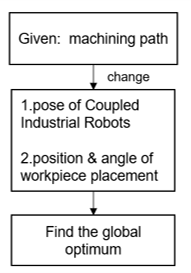
\includegraphics[width=\textwidth]{03_images/process.png}
	\caption{Graphical representation of the research process.}
	\label{fig:Introduction:meme}
\end{figure}






	\cleardoublepage
	\chapter{Fundamentals} \label{ch:Fundamentals}

In this chapter...
	\cleardoublepage 
	\chapter{Global optimization scheme} \label{ch:scheme}
In Chapter 1, it is introduced that optimizing the stiffness of the coupling robot in the manufacturing process can improve the manufacturing accuracy of the workpiece. The comparison and analysis of optimization methods through Chapter 2, the choice of using particle swarm optimization method to improve the stiffness of physically coupled robots in the manufacturing process. This chapter presents the development of a global optimization scheme for enhancing stiffness.
\section{Machining Process} \label{sec:scheme:process}
\subsection{Machining Path} \label{subsec:sec:scheme:process:path}
Machining is a process in which a material is cut to a desired final shape and size by a controlled material-removal process. The three principal machining processes are classified as turning, drilling and milling. The machining path is the path through space that the tip of a cutting tool follows to produce the desired geometry of the workpiece. The physically coupled robots perform coordinated machining tasks. Various machining tasks, such as drilling and milling, can be implemented if tools are attached to the coupler. 
\subsubsection{Path generation} \label{subsubsec:subsec:sec:scheme:process:path: path generation}
The given machining path is converted according to the G-code. G-code is the most widely used computer numerical control (CNC) programming language \cite{cncs}. It is used mainly in computer-aided manufacturing to control automated machine tools and has many variants. Extensions and variations of G-code have been added independently by control manufacturers and machine tool manufacturers, and operators of a specific controller must be aware of the differences between each manufacturer's product. In CNC machining centers, the G-code is composed of the letter G and two digits and is used for the control of tool paths, i.e., the movement of each feed axis, such as linear or arc interpolation, feed control, offset and transformation of the origin of the coordinate system, setting of dimensional units, tool offset and compensation. \par
The machining path can be generated using a combination of lines and arcs as the basic elements according to the G-code introduction above \cite{dqt}. Each element has a starting phase (velocity from zero to a constant value) and an ending phase (velocity from a constant value to zero). The basic elements overlap in their transition phases so that a line can be smoothly connected to an arc with a continuous position and velocity \cite{dqt}. \par
A $\boldsymbol{timeframes} = (t_{i,j})_{n \times 4}$ can represent the relationship between a given machining path and time. $t_{i,1}$ represents the time value in the i-th element corresponding to a speed of zero in the starting phase, $t_{i,2}$ represents the time value in the i-th element corresponding to a speed of a constant value in the starting phase, $t_{i,3}$ represents the time value in the i-th element corresponding to a speed of a constant value in the ending phase and $t_{i,4}$ represents the time value in the i-th element corresponding to a speed of zero in the ending phase. n represents a machining path with n basic elements. $\boldsymbol{timeframes}$ can be shown as follows:
\begin{equation}
\boldsymbol{timeframes} = \begin{bmatrix} 
    t_{1,1} & \dots  & b_{1,4}\\
    \vdots & \ddots & \vdots\\
    b_{n,1} & \dots  & b_{n,4} 
    \end{bmatrix}
    \label{eq:tframe}
\end{equation}
According to the path characterization, there is a special relationship between $t_{i,3}$ and $t_{i+1,1}$, $t_{i,4}$ and $t_{i+1,2}$. As the acceleration phase corresponding to each element and the deceleration phase corresponding to the last element are fitted to the final machining path, the time values $t_{i,3}$ and $t_{i+1,1}$, $t_{i,4}$ and $t_{i+1,2}$ are averaged as the characteristic time points of the sampling points. Then, based on the matrix (\ref{eq:tframe}), the following vector $\boldsymbol{t_{\mathrm{characteristic}}}$ generated from the characteristic time points can be obtained. In the same way, this vector is the key data for the next step of data processing.
\begin{equation}
  \boldsymbol{t_{\mathrm{characteristic}}} =  \begin{bmatrix}
       t_{1,1} & \frac{t_{1,3}+t_{2,1}}{2} & \frac{t_{1,4}+t_{2,2}}{2} &  & \dots & \frac{t_{n-1,3}+t_{n,1}}{2} & \frac{t_{n-1,4}+t_{n,2}}{2} & t_{n,4} \end{bmatrix}^\top
       \label{eq:tcha}
\end{equation}
\subsection{Data Pre-processing} \label{subsec:sec:scheme:process:Data Pre-processing}
The challenge of enhancing stiffness is finding the stiffest configurations along the entire path, not at a single point. That means the coupled robot needs to move along a predefined machining path to ensure that the actual machining path matches the predefined path. The path is on the workpiece, and the workpiece can be placed freely in the space. In addition, evaluating and optimizing robots' configurations along a continuous machining path are time-consuming, so data pre-processing is needed to reduce the computation.
% \subsubsection{Choice of sampling method}\label{subsubsec:subsec:sec:scheme:process:Data Pre-processing:sampling method}
Data pre-processing, in other words, is the use of a sampling method to extract sample points. Commonly used sampling methods are equal distance sampling and equal time interval sampling. As the sampling methods listed previously do not consider information about the characteristics of the machining path, such as straight lines or curves, they increase the number of sampling points. Therefore, the more computational effort is required to complete the optimization process later. \par
In order to better take into account the feature information of the path points and to reduce the number of sampling points, resampling will be performed based on the above obtained time-dependent characteristic vector $\boldsymbol{t_{\mathrm{characteristic}}}$. The vector is shown as (\ref{eq:tcha}). \par
Firstly, introduce the resampling and its sampling process. The resampling is based on the data obtained from the previous matrix $\boldsymbol{t_{\mathrm{characteristic}}}$ relating to time, removing some unnecessary points to reduce the number of sampled points. \par
The resampling process is as follows:
\begin{itemize}
 \item \textbf{Step 1}: There is a series of points on the curve: $p_{0},p_{1}...p_{n-1},p_{n}$, as shown in
Figure \ref{fig:main:sampling1}. $p_{0}$ represents the path point under the time value corresponding to the first element of the vector $\boldsymbol{t_{\mathrm{characteristic}}}$, $p_{1}$ represents the second element, and so on. $p_{n}$ refers to the path point of the last element.
\item \textbf{Step 2}: Calculate the distance of $p_{1},p_{2}...p_{n-1}$ to the line $p_{0},p_{n}$ as shown in Figure \ref{fig:main:sampling2}.
\item \textbf{Step 3}: Find the maximum value of distance $p_{k}$, as shown in
Figure \ref{fig:main:sampling3}.
\item \textbf{Step 4}: If $p_{k}\leq d_\mathrm{tolerance}$, save $p_{0},p_{n}$ two points is sufficient. Else divide into two polylines at the point where $p_{k}$ is located and go to Step 2. $d_\mathrm{tolerance}$ is the required sampling tolerance.
\end{itemize}
\begin{figure}[h!]
\centering
\vspace{-1cm}
\setlength{\abovecaptionskip}{-1cm} 
\begin{minipage}[t]{0.48\textwidth}
\centering
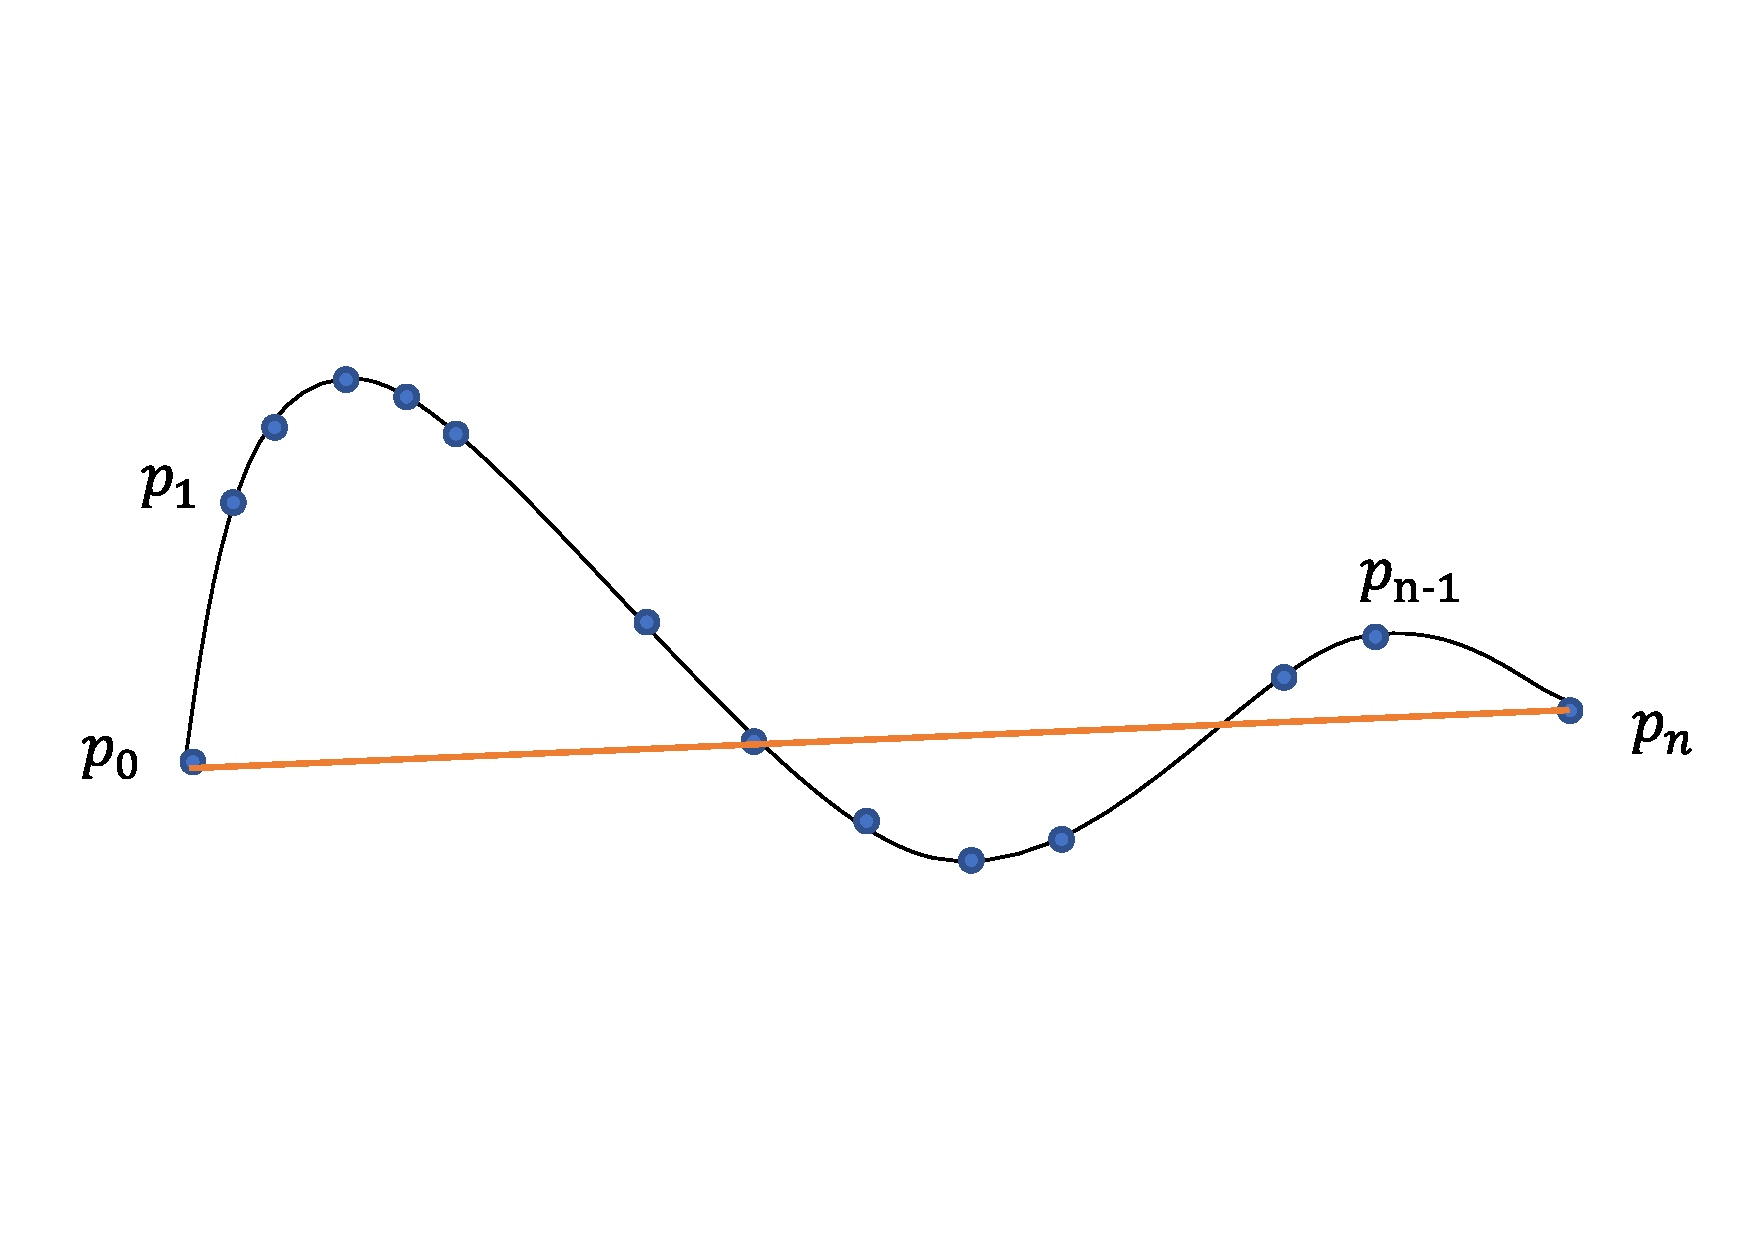
\includegraphics[width=6cm]{03_images/sampling_1.pdf}
\caption{Step 1}
\label{fig:main:sampling1}
\end{minipage}
\begin{minipage}[t]{0.48\textwidth}
\centering
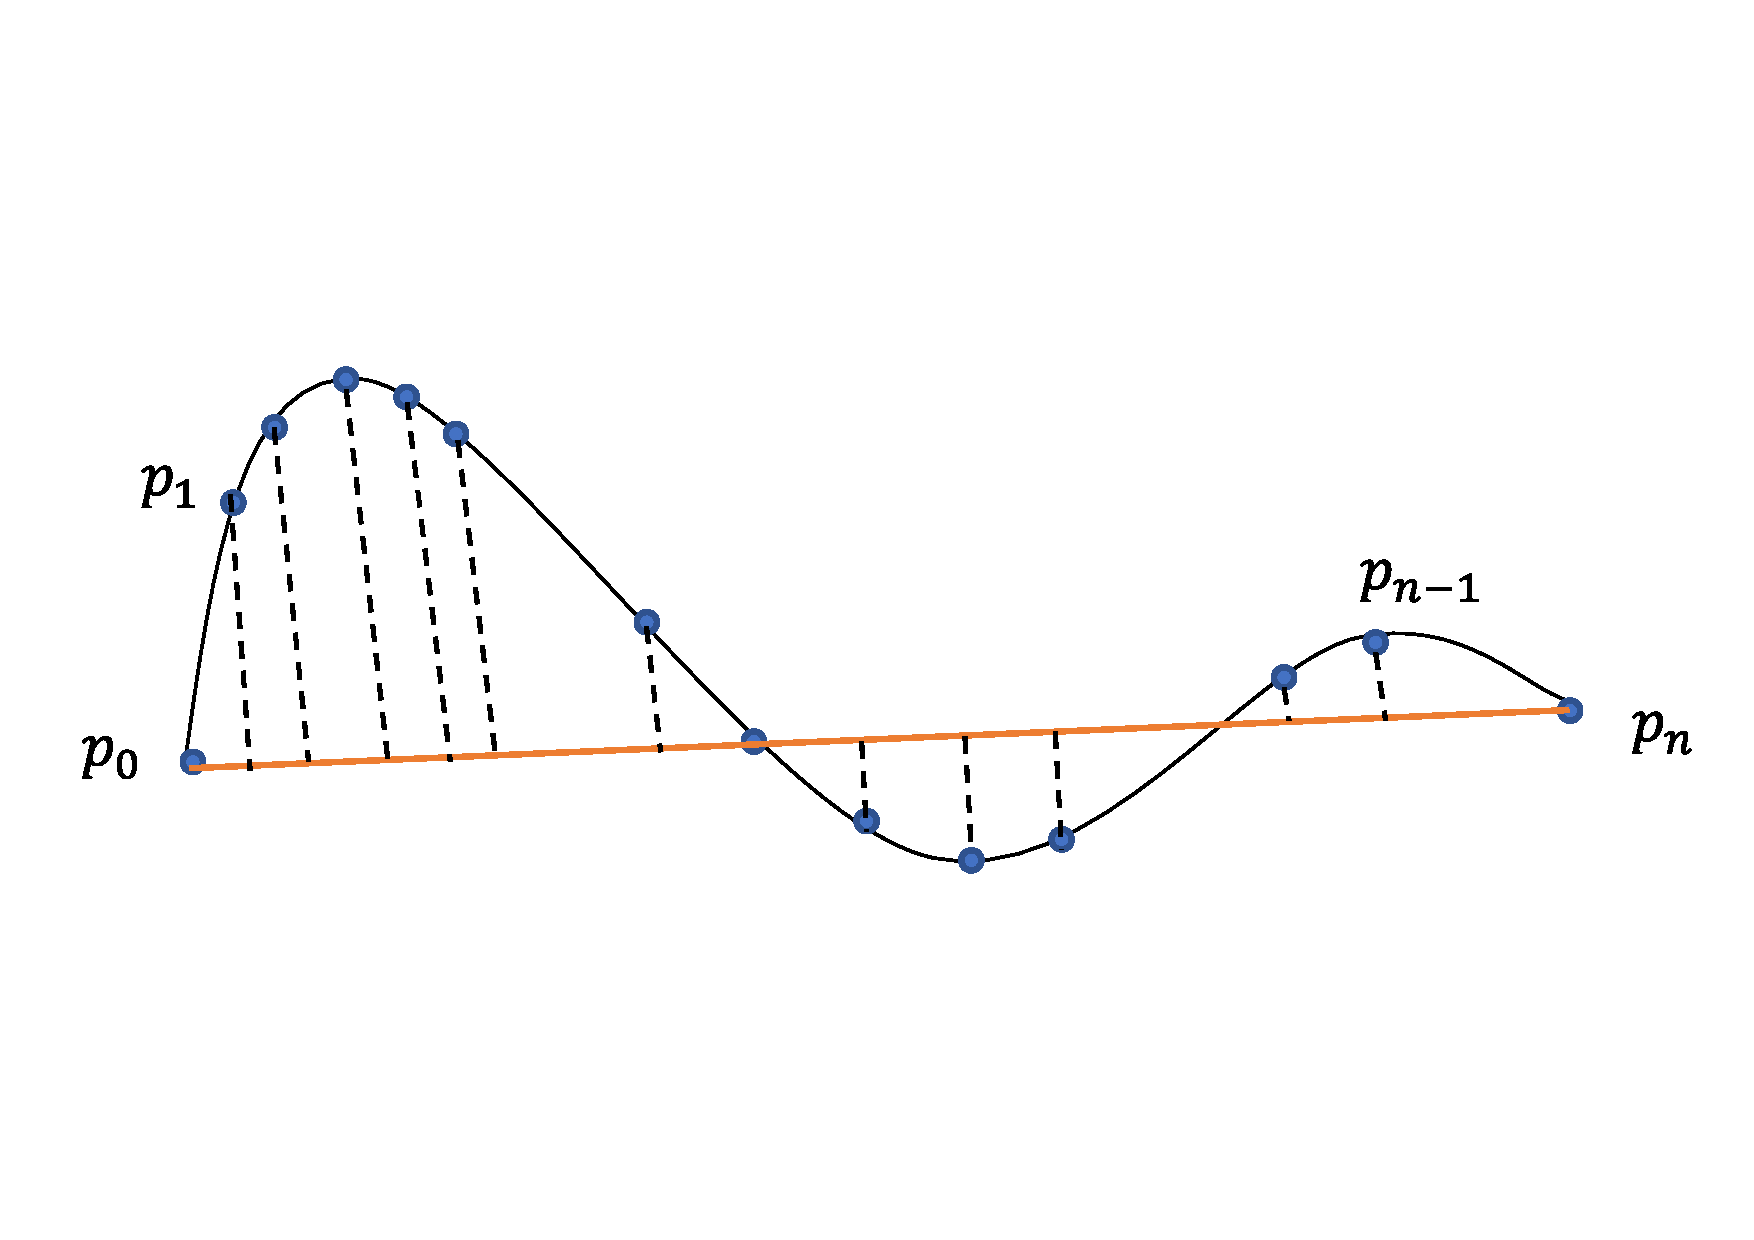
\includegraphics[width=6cm]{03_images/sampling_2.pdf}
\caption{Step 2}
\label{fig:main:sampling2}
\end{minipage}
\end{figure}
\begin{figure}[h!]
	\centering
        \vspace{-1.7cm}
        \setlength{\abovecaptionskip}{-1cm}
	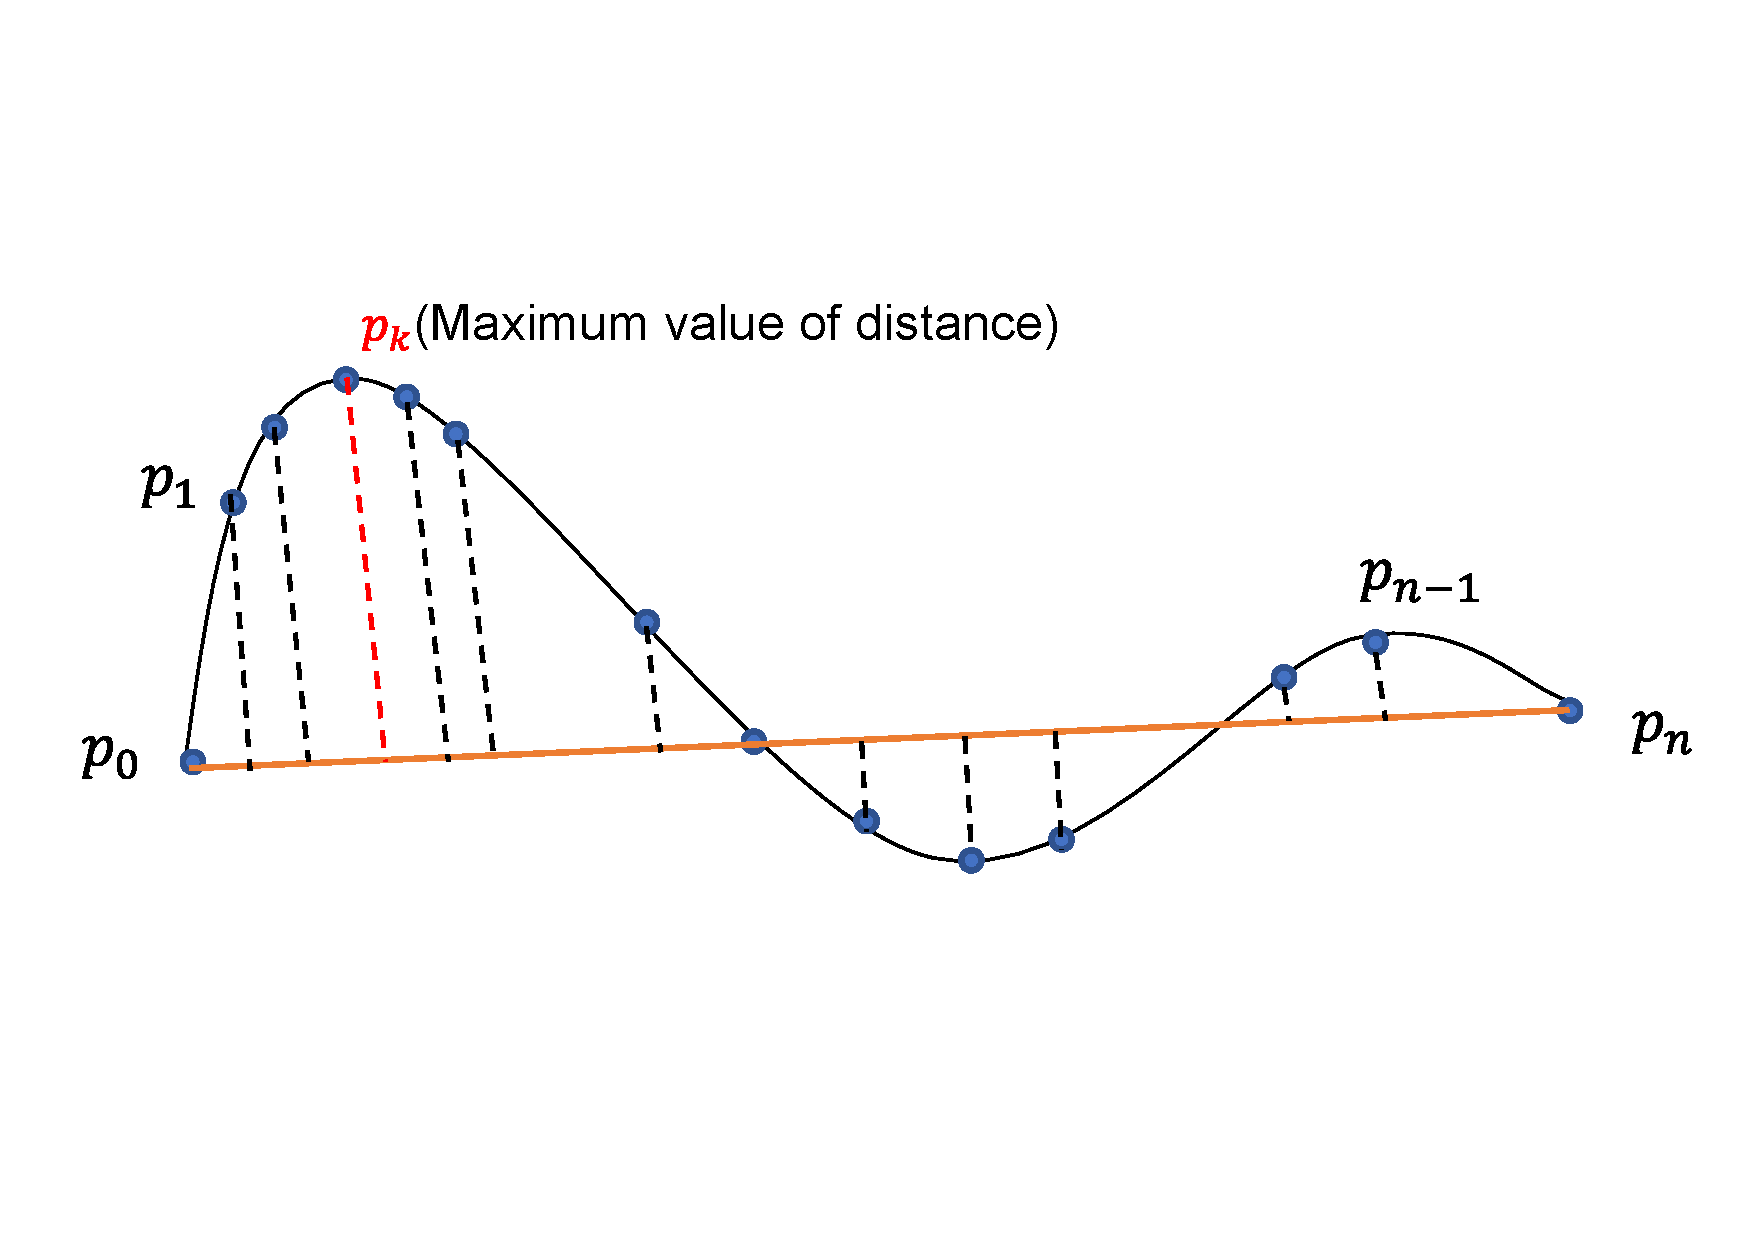
\includegraphics[width=6cm]{03_images/sampling_3.pdf}
	\caption{Step 3}
	\label{fig:main:sampling3}
\end{figure}
% \subsection{Acquisition of sampled points for machining path }\label{subsec:sec:Main:Pre-processing:sampled points}
Based on the introduction of the resampling steps, the following will explain how resampling is applied to the data pre-processing process.\par
Before applying resampling to the data pre-processing, it needs to be determined how step 2 above calculates the point-to-line distance as in equation (\ref{eq:cald}). 
\begin{equation}
   d_{i} = \frac{\left|(p_{i}-p_{0}) \times (p_{i}-p_{n})\right|}{\left|(p_{n}-p_{0})\right|} 
\label{eq:cald}
\end{equation}
$p_{i}$ represents a point apart from the first and last points on the path, $p_{0}$ represents the first point of the path, and $p_{n}$ represents the last point. \par
\begin{algorithm}
\SetAlgoLined
\caption{Resampling} \label{alg1} 
\KwData{The relationship between a given machining path and time: $\boldsymbol{timeframes} \in \mathbb{R}^{n\times4}$,\;
Time-dependent characteristic vector: $\boldsymbol{tcha}$,\;
Time corresponding to the start point of the currently analysed part of the machining path: $t_\mathrm{start}$, \;
Time corresponding to the end point of the currently analysed part of the machining path: $t_\mathrm{end}$, \;
Minimum value of the time interval between two points: $\epsilon$,\;
Sampling tolerance: $d_\mathrm{tolerance}$}
\KwResult{Matrix of the times corresponding to the sampled points after resampling: $\boldsymbol{sample_{\mathrm{path}}}$ }
$t_\mathrm{start}\gets \boldsymbol{tcha}_{1}$;\;
$t_\mathrm{end}\gets \boldsymbol{tcha}_{2}$;\;
$\boldsymbol{sample_{\mathrm{path}}} \gets \left[ \right]$;\;
\While{$\boldsymbol{tcha} \neq \varnothing $}{
    \eIf{$\boldsymbol{tcha}$ contains only one element}{
    Add $\boldsymbol{tcha}_{1}$ to the last element of the matrix $\boldsymbol{sample_{\mathrm{path}}}$; \;}
      {\If{$t_\mathrm{end} - t_\mathrm{start} > \epsilon$}{
      $\boldsymbol{d} \gets \left[ \right]$;\;
      \tcp{$\boldsymbol{d}$ is a vector that stores the distance from the path point to the line connected to the first and last except for the first and last two points}
      \While{$t_\mathrm{start}<t_{i}<t_\mathrm{end}$}{
       Calculate $d_{i}$;\;
       Add $ d_{i}$ to the last element of the matrix $\boldsymbol{d}$;\;
       $ t_{i} \gets t_{i}+ \epsilon$;}
        }
      {\eIf{$\max\boldsymbol{d} > d_\mathrm{tolerance}$} 
        {Divide into two polylines at the point where $\max\boldsymbol{d}$ is located;}
        {Add $\begin{bmatrix}
         t_\mathrm{start} & t_\mathrm{end}
         \end{bmatrix}^\top$ to the last element of the matrix $\boldsymbol{sample_{\mathrm{path}}}$;\;
        Delete $\boldsymbol{tcha}_{1}$;\;
        $t_\mathrm{start}\gets \boldsymbol{tcha}_{1}$;\;
        $t_\mathrm{end}\gets \boldsymbol{tcha}_{2}$;}}
        }
        }
\end{algorithm}
% As shown in the Figure \ref{fig:main:samplepoints}, the shape after resampling can be seen as the same as the original curve, but the resampling only requires eleven sampling points.
% \begin{figure}[h!]
% 	\centering
%         \vspace{-3cm}
%         \setlength{\abovecaptionskip}{-7.5cm}
% 	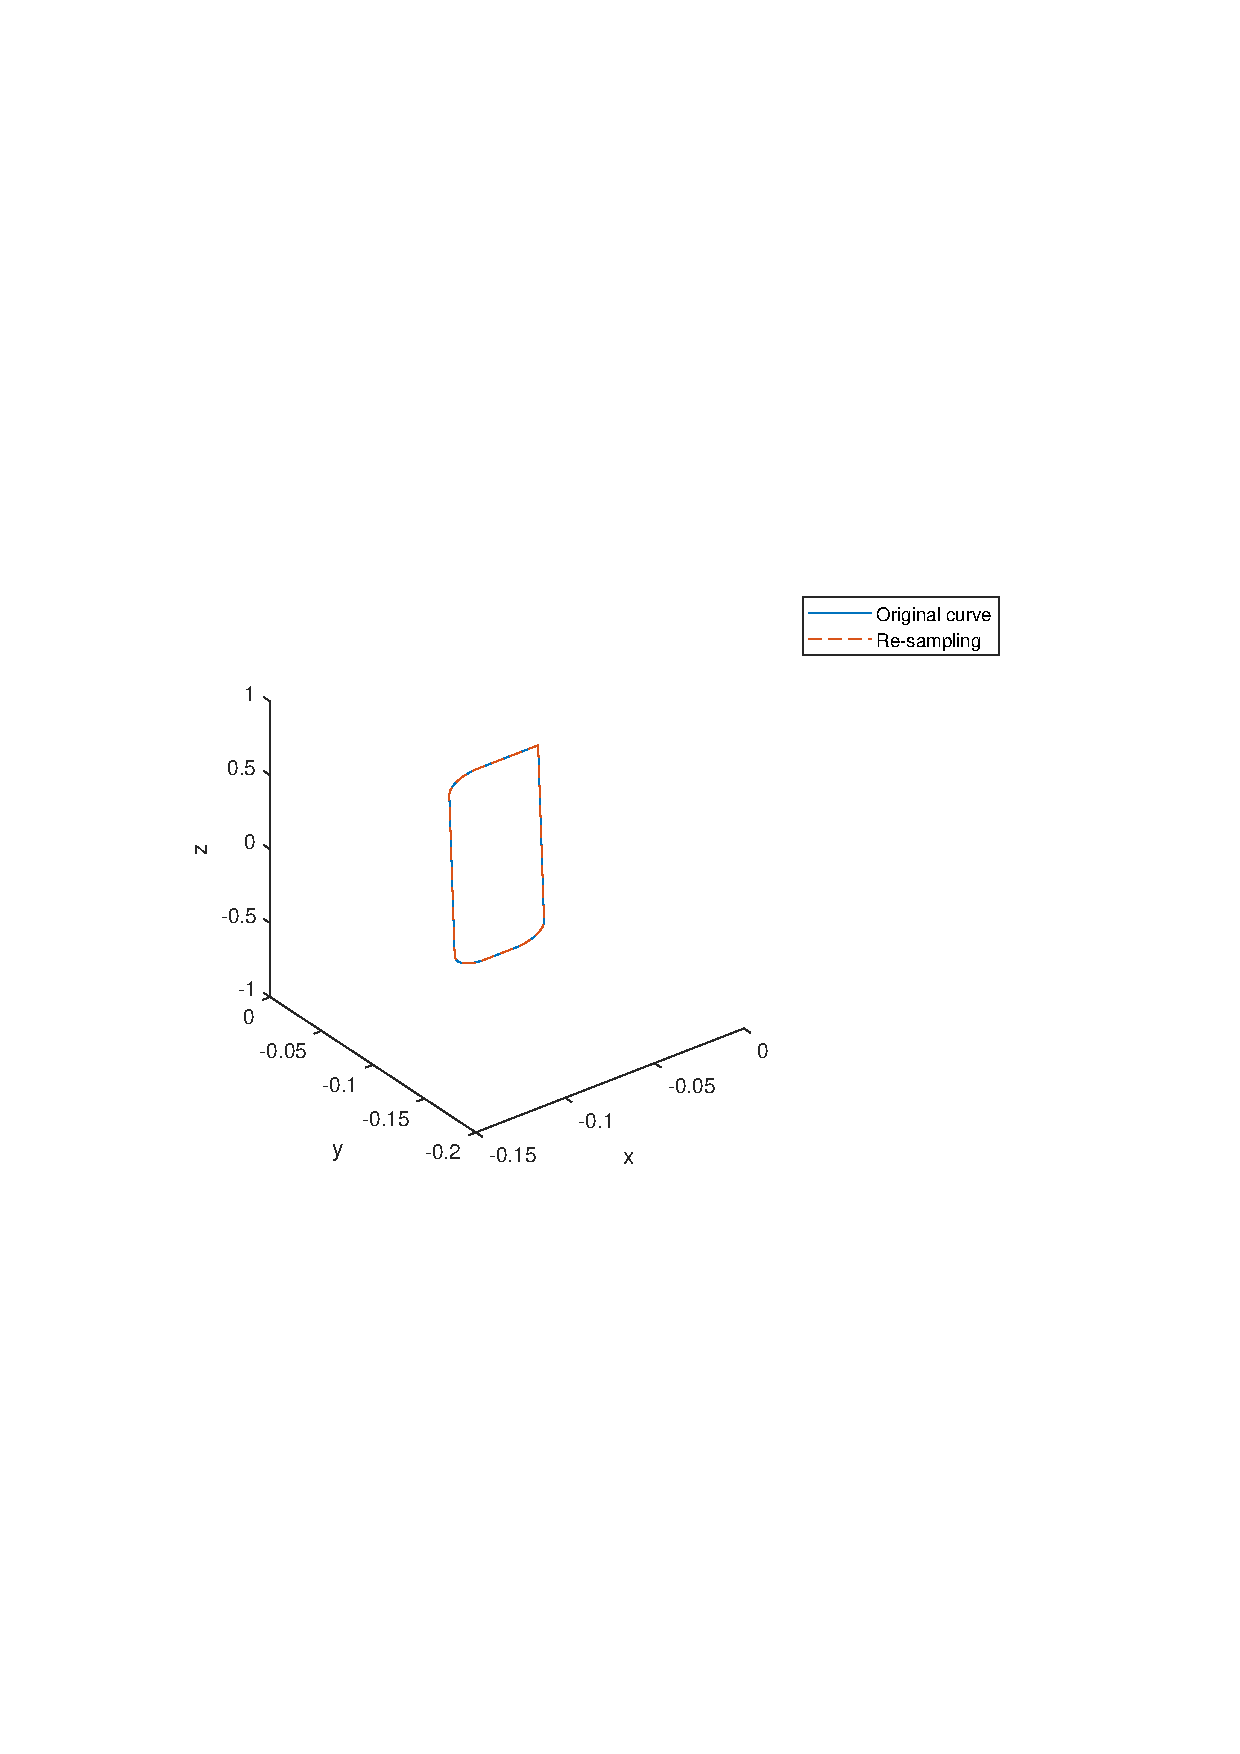
\includegraphics[width=\textwidth]{03_images/sample_point.pdf}
% 	\caption{Comparison of original and resampling curves}
% 	\label{fig:main:samplepoints}
% \end{figure}
\section{Physically couppled robot} \label{sec:scheme:robot}

        \cleardoublepage 
	\include{02_chapter/04_.tex}
        \cleardoublepage 
	\include{02_chapter/05_.tex}
%	\printbibliography
	%% ---------------------------------------------------------------------------
	%% Appendices
	%% ---------------------------------------------------------------------------
	
	\begin{appendix}
		\cleardoublepage
		\chapter{Trivial Proofs}

The following sections demonstrate the veracity of Figure~\ref{fig:Introduction:meme} and \eqref{eq:Introduction:realisation}.

\section{Central Argument}

Patrick is a genius.

\section{Motivation}

Careful observation.

\section{Listings}

Quellcodes lassen sich gut mit dem listings-Paket einbinden, so ist das Einbinden von entsprechend formatiertem Matlab-/C++/etc.-Code ohne Copy/Paste direkt aus der Quellcode-Datei möglich. Und hier noch ein Beispielhafter Matlab Quellcode:

\begin{lstlisting}[caption={Ein wahnsinnig komplizierter Quellcode}]
	%% State Space System
	asyn.SS = ss(asyn.A,asyn.B,asyn.C,asyn.D);
	
	% Infos über das System
	disp('- Informationen über das System -');
	% Ordnung des Systems
	asyn.n = rank(asyn.A);
	disp(['Ordnung des Systems n = ', num2str(asyn.n)]);
	% Polstellen
	asyn.PS = pole(asyn.SS);
	% Nullstellen
	asyn.NS = tzero(asyn.SS);
	% Beobachtbarkeit
	asyn.Ob = obsv(asyn.SS);
	if rank(asyn.Ob) == asyn.n
	disp('System vollständig Beobachtbar');
	else
	disp('System nicht vollständig Beobachtbar');
	end
	% Steuerbarkeit
	asyn.Os = ctrb(asyn.SS);
	if rank(asyn.Os) == asyn.n
	disp('System vollständig Steuerbar');
	else
	disp('System nicht vollständig Steuerbar');
	end
	
	disp('---------------------------------');
\end{lstlisting}
	\end{appendix}
	
	%% ---------------------------------------------------------------------------
	%% ---------------------------------------------------------------------------
	
	% Listings - remove if not required
	\cleardoublepage
	\lstlistoflistings % Requires the listings package
	
	% Algorithms - remove if not required
	\cleardoublepage
	\listofalgorithms % Requires the either "algorithm2e" or "algorithms" packages
	\addcontentsline{toc}{chapter}{List of algorithms}

	\cleardoublepage
	\pagenumbering{Roman}
	\printbibliography


	
%	\bibliography{04_bib/bib}
%\nocite{*}
%\bibliography{04_bib/literature} 
	
\end{document}